\documentclass{article}

\usepackage[utf8]{inputenc}
\usepackage{hyperref}
\usepackage{listings}
\usepackage{graphicx}
\usepackage{listings}

\title{Lab Sheet 3}
\date{Security}

\begin{document}
\maketitle

In our third lab, we will use \href{https://www.cyberpunk.rs/password-cracker-thc-hydra}{hydra}, a tool in Kali Linux, to perform a Brute Force attack on a Web based login. Hydra is the fastest network logon cracker which supports numerous attack protocols. It is very fast and flexible, and new modules are easy to add. This tool makes it possible for researchers and security consultants to show how easy it would be to gain unauthorized access to a system remotely. 

\section{Task 1: Brute Force Web-based Login with hydra}
We will use http to run a brute force attack on a vulnerability testing site.

\subsection{Get to know your tool}
Type \texttt{hydra -h} (\texttt{h} for help) in your Kali terminal and find out what \textit{hydra} is all about and how it might work.

\subsection{Intro}
One of hydra's brute force attacking services is used on Web-based logins, such as social media login forms, user banking login forms, your router's Web-based login, etc. That's \texttt{http[s]-{get|post}-form} which will handle this request.

Before we fire up hydra, we should know some of the arguments:
\begin{itemize}
\item \textbf{Target:} http://testasp.vulnweb.com/Login.asp?RetURL=\%2FDefault\%2Easp\%3F
\item \textbf{Login username:} admin (if you're not sure, bruteforce this)
\item \textbf{Password list:} ``The location of the dictionary file list containing possible passwords.''
\item \textbf{Form parameters:} ``Here we will be using iceweasel or firefox network developer toolbar.''
\item \textbf{Service module:} http-post-form
\end{itemize}

\subsection{Obtaining post parametres}
Visit \href{http://testasp.vulnweb.com/Login.asp?RetURL=\%2FDefault\%2Easp\%3F}{http://testasp.vulnweb.com/Login.asp?RetURL=\%2FDefault\%2Easp\%3F} and open the \textit{Network} tool in the \textit{Web Developer} menu.

To obtain the post-form parameters, type anything in the \textit{username} and/or \textit{password} form. You will notice a new \textbf{POST} method on the network developer tab. Click on that line and on the \textit{Headers} tab click \textit{Edit and Resend} on the right side. From the \textit{Request Body} textbox, copy the last line, e.g. \texttt{tfUName=admin\&tfUPass=password}. The \textit{tfUName} and \textit{tfUPass} are parameters we need (see Figure 1).

\begin{figure}[h]
  \centering
  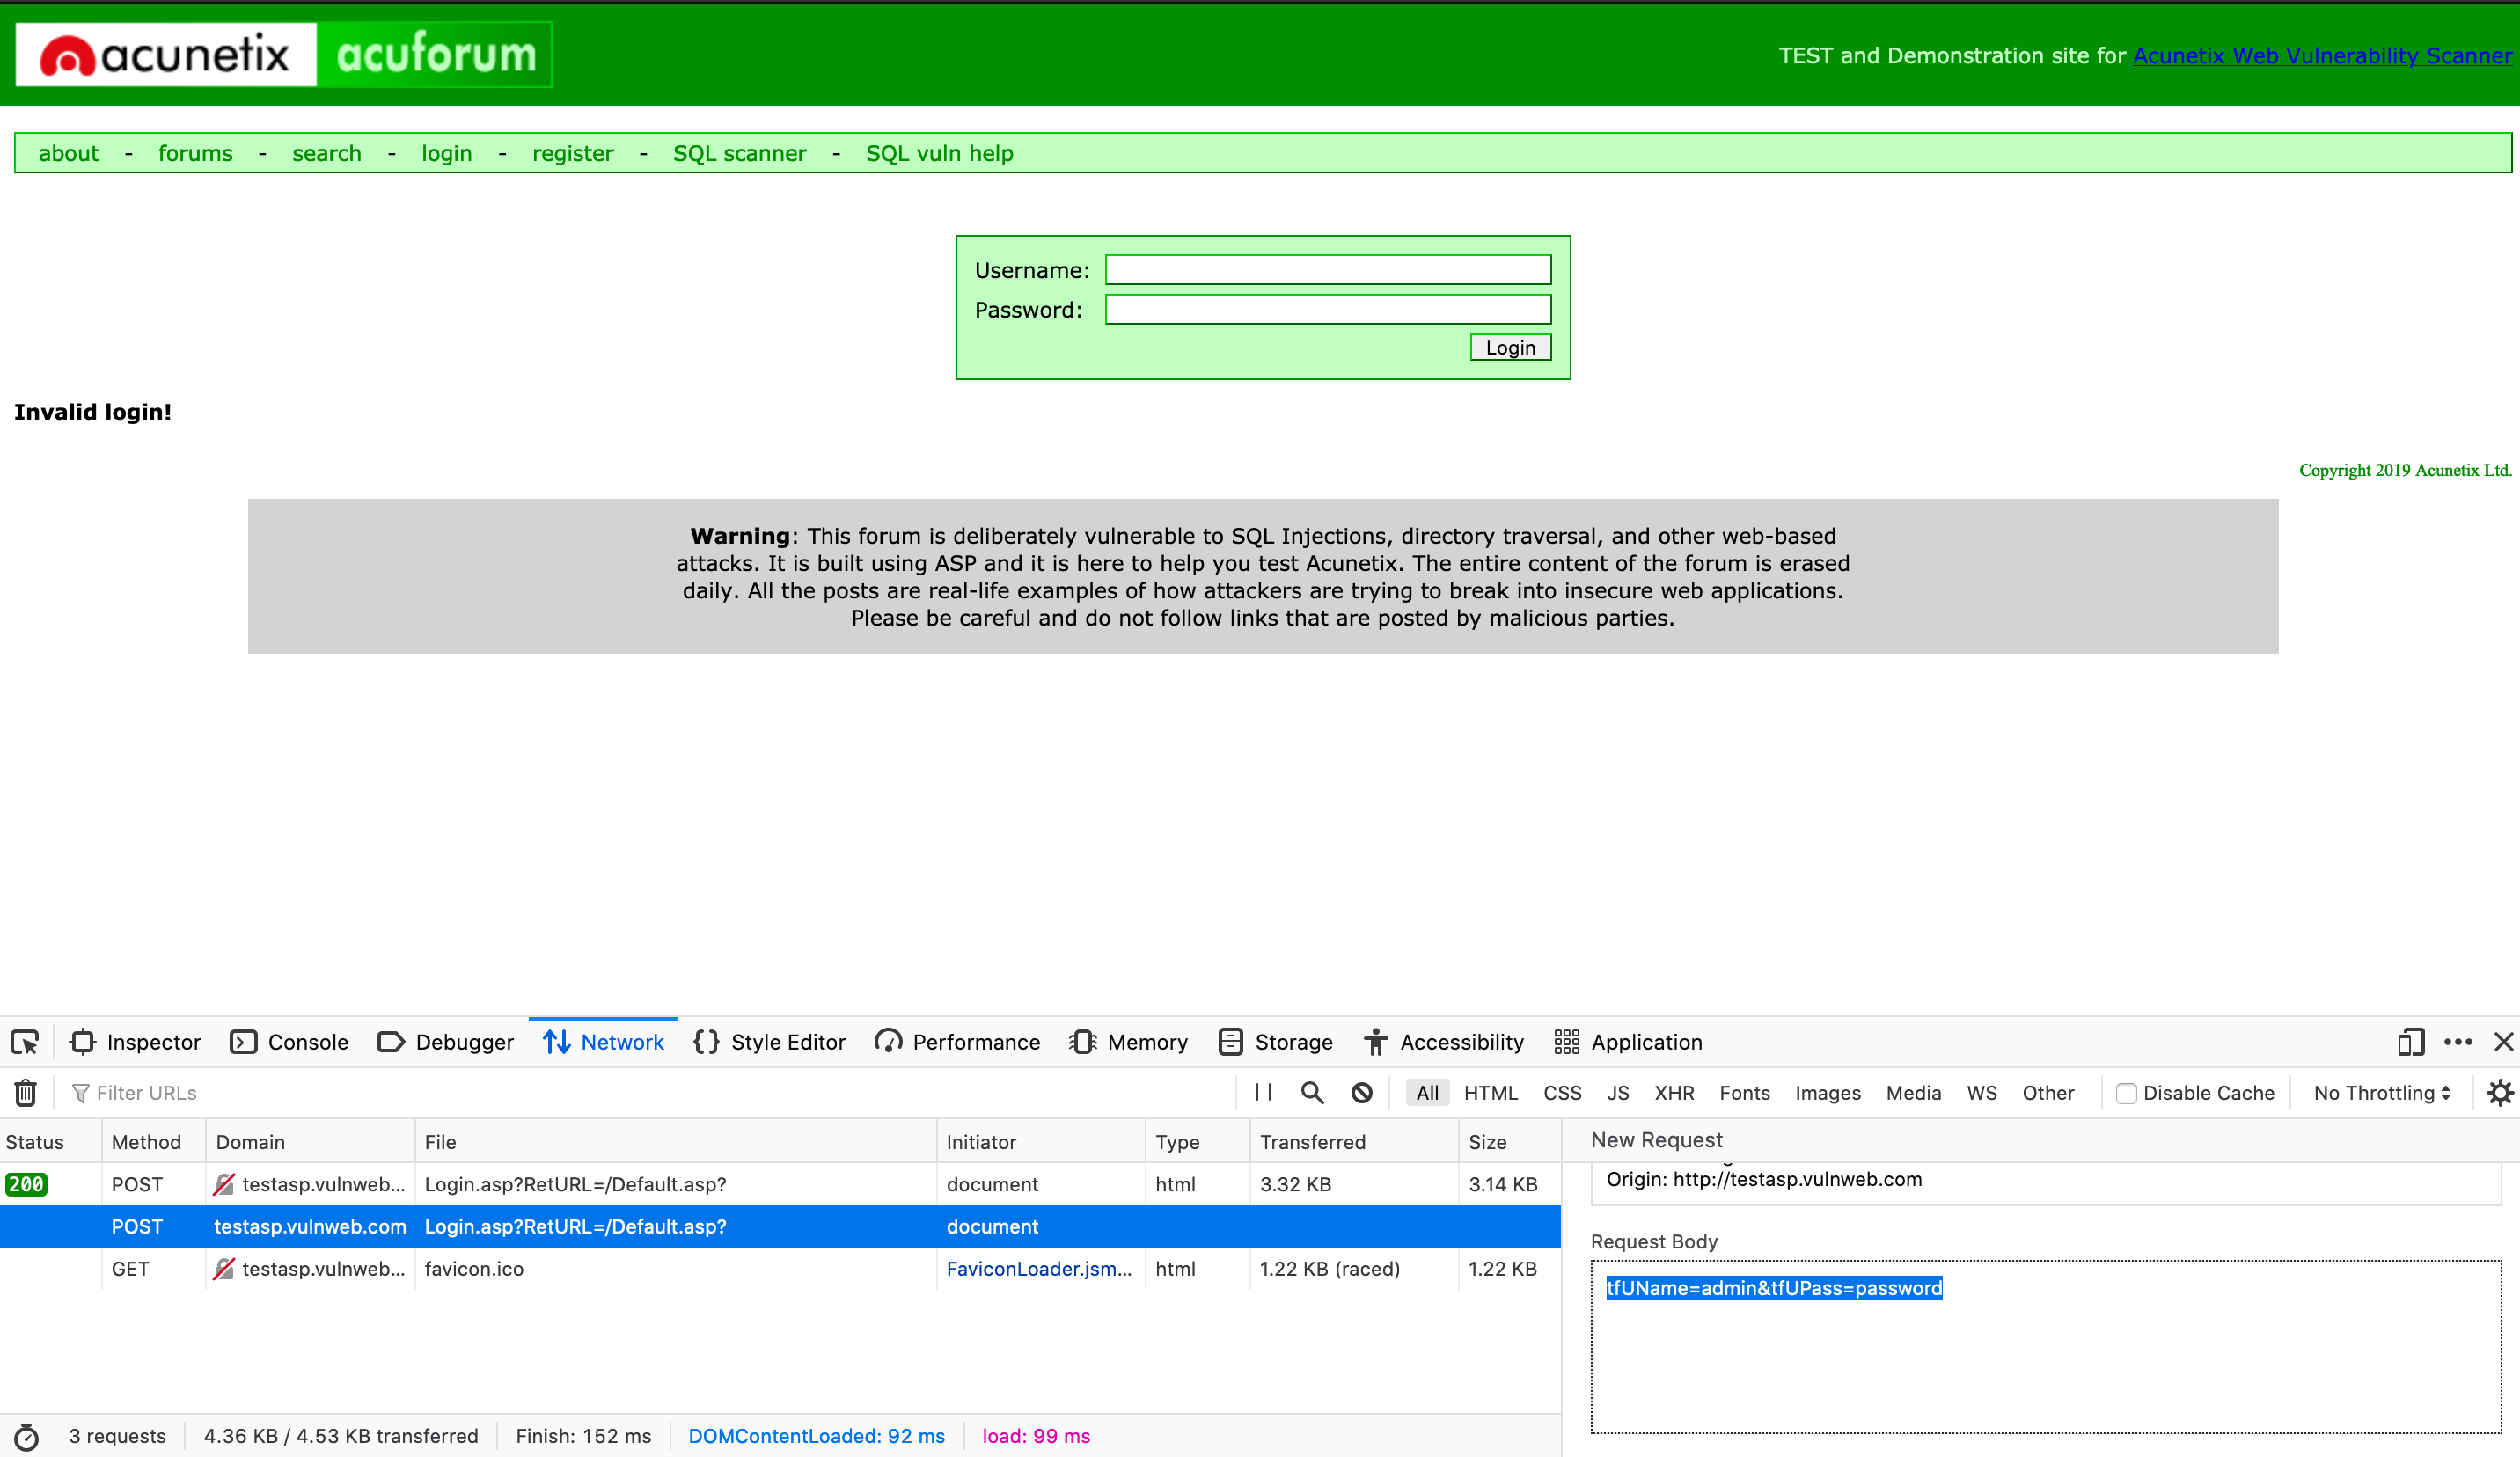
\includegraphics[width=12cm]{request-body}
  \caption{Copying Request Body.}
\end{figure}

\subsection{Wordlists}
Kali Linux has a bunch of wordlists, so you can choose the appropriate one or just use rockyou.txt from \texttt{/usr/share/wordlists/}. So copy the worlist into your home directory and use \textit{gzip} to unzip the archive. Type \texttt{cat rockyou.txt} to see how many passwords the wordlist contains.

\subsection{Run the attack}
Alright, now that we got all arguments, we are ready to fire up hydra. Here is the command pattern:
\begin{lstlisting}
  hydra -l <username> -P <password list> <Target hostname>
  <service module>  <post request parameters>[/code]
\end{lstlisting}
Based on information we have gathered, our command should look something like this:
\begin{lstlisting}
  hydra -l admin -P /usr/share/wordlists/rockyou.txt
  testasp.vulnweb.com http-post-form
  "/Login.asp?RetURL=%2FDefault%2Easp%3F:tfUName=
  ^USER^&tfUPass=^PASS^:S=logout" -vV -f
\end{lstlisting}
Let’s break down the commands:
\begin{itemize}
  \item \textbf{-l $<$username$>$:} user name (not hard to guess), use -L $<$FILE$>$ for a list of possible user names from a file.
  \item \textbf{-P $<$FILE$>$:} file with passwords, use -p $<$password$>$ to literally use one password instead of guessing it.
  \item \textbf{testapp.vunlwebapp.com:} is a hostname or target.
  \item \textbf{http-post-form:} is the service module we use.
  \item \textbf{/Login.asp?...} This is  \{page URL\}:\{Request post body form parameters\}:S=\{Find whatever on the page after succesfully logged in\}.
   \item \textbf{v:} Verbose mode.
   \item \textbf{V:} Show \textit{login:pass} for each attempt.
   \item \textbf{f:} Terminate program if pair \textit{login:password} is found.
\end{itemize}
Now just run the command and watch the terminal output.

\section{Task 2: Cracking LinkedIn Hashes Using Hashcat}
In this section, you'll see how many hashes you can recover from the 2016 LinkedIn password breach. The LinkedIn hacker, a Russian, was sentenced in US court to seven years in jail on September 29, 2020. This breach of 177,500,189 unsalted SHA1 password hashes represents the data of all LinkedIn users as of 2012. Among these passwords, only 61,829,207 are unique.

In this lab you will only crack 500,000 hashes, so we'll do the following:
\begin{enumerate}
\item Download a copy of the file \href{https://raw.githubusercontent.com/deargle/security-assignments/master/labs/files/LinkedIn\_HalfMillionHashes.txt}{LinkedInHalfMillionHashes.txt}. (use \textit{wget}.
\item To get your feet wet, perform a ''straight'' dictionary attack using the \textit{rockyou.txt} wordlist again. This attack will try each entry in the rockyou dataset with no permutations.
\item Read the man page for \textit{hashcat} to make sure you know what the switches do and the nrun \texttt{hashcat --force -m 100 --remove --outfile=LinkedIn\_cracked.txt LinkedIn\_HalfMillionHashes.txt}
\item To see how many you cracked so far, run: \texttt{wc -l LinkedIn\_cracked.txt} or number of passwords left with: \texttt{wc -l LinkedIn\_HalfMillionHashes.txt}
\end{enumerate}

\section{Task 3: Create a Targeted Wordlist Using CeWL}
CeWL (Custom Word List Generator) is a command-line tool that creates custom wordlists from a target website. This can be useful for cracking a password of an organization or individual that also has a website or social media profile. Because people often use information about themselves or their organization when creating passwords, custom wordlists can be very effective.

Imagine that you exfiltrated the following MD5 hash from a database:
\begin{lstlisting}
cf4aff530715824c055892438a1ab6b2
\end{lstlisting}
You want to create a custom dictionary using the words on \href{neurosecurity.byu.edu}{neurosecurity.byu.edu} to see if you can crack the hash.
\begin{enumerate}
\item Create a custom dictionary using CeWL for the website neurosecurity.byu.edu (again check the arguments on the manpage): \texttt{cewl -v -d 2 -m 5 -w custom\_dict.txt https://neurosecurity.byu.edu}
\item Check how many entries are in the \textit{custom\_dict.txt} file: \texttt{wc -l custom\_dict.txt}
  \item Look at the words in \textit{custom\_dict.txt}: \texttt{less custom\_dict.txt}
  \item Permute the words in the \textit{custom\_dict.txt} wordlist using the ''best64'' rule, and append the output to \textit{custom\_dict.txt} (all one line): \texttt{hashcat custom\_dict.txt -r /usr/share/hashcat/rules/best64.rule --stdout $>>$ custom\_dict.txt}
    \item Check how many entries are in the \textit{custom\_dict.txt} file now: \texttt{wc -l custom\_dict.txt}
    \item Run Hashcat using \textit{custom\_dict} against the MD5 hash (all one line): \texttt{hashcat --force -a 0 -m 0 cf4aff530715824c055892438a1ab6b2 custom\_dict.txt} Where \textit{-m 0} signifies md5 mode, and \textit{-a} specifies ''straight attack mode'' (do not permutate the wordlist, because we already did). The password will be reported towards the top of the output in the format: \textit{hash:password}. If you miss the output, you can view it in your potfile once you have cracked it by running: \texttt{hashcat --show cf4aff530715824c055892438a1ab6b2}
    \item Confirm that you found the correct password: \texttt{echo -n ''$<$the plaintext password$>$'' $|$ md5sum} We include the \textit{-n} flag because otherwise, the echo command will append a newline character, which will throw off the hash.
\end{enumerate}

\end{document}
